\section{Desenvolvimento do metamodelo}

O metamodelo final foi definido com 14 parâmetros:
\begin{itemize}
	\item Fator de abertura das janelas;
	\item Velocidade do ar;
	\item Condição de exposição das paredes e janelas;
	\item Área da sala;
	\item Densidade de ocupação;
	\item Altura do pavimento;
	\item Exposição da cobertura;
	\item Sombreamento horizontal;
	\item Contato com o solo;
	\item Transmitância das paredes;
	\item Absortância das paredes;
	\item Fator solar do vidro;
	\item Azimute da sala;
	\item \Acrlong{paf}.
\end{itemize}

As 100.000 simulações termoenergéticas foram desenvolvidas para o treinamento da rede neural artificial (\acrshort{ann}) a partir de combinações entre os parâmetros definidos.
Os parâmetros variaram na mesma faixa de valores estabelecida na Seção \ref{section:parametrosdeentrada}. O ângulo do azimute da sala é determinado considerando-se o eixo entre a parede voltada para a circulação e a parede oposta à circulação.
O contato com o solo e a exposição da cobertura foram definidas como variáveis binárias, com o valor zero correspondendo à superfície adiabática, e 1 correspondendo à exposição.
O parâmetro que representa a condição de exposição das paredes e janelas não foi representado com valores numéricos, e sim como uma variável de fatores, com cinco opções de exposição. Além das três opções apresentadas na Figura \ref{fig:exp_sz}, considerou-se também as exposições espelhadas. 	
Os demais parâmetros foram normalizados com valores entre -1 e 1.

\begin{figure}[h]
	\centering
	\caption{Condição de exposição das paredes e janelas}
	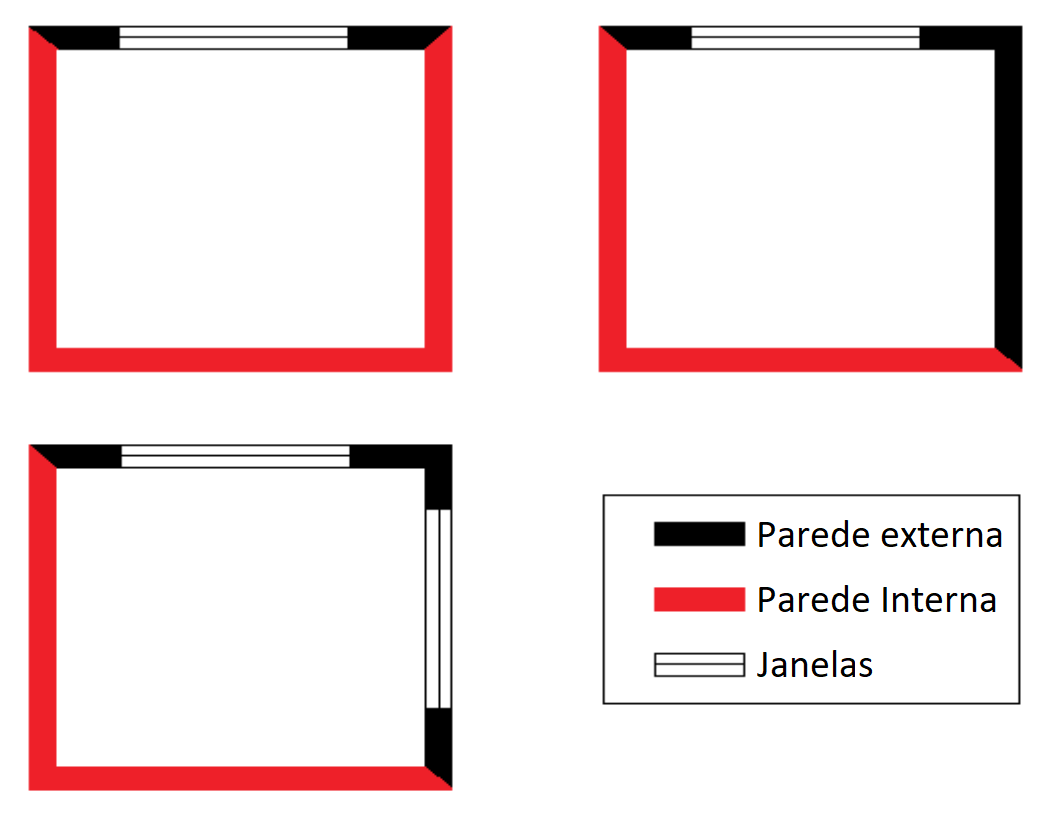
\includegraphics[width=.5\linewidth]{img/wallexposition2.png}
	\label{fig:exp_sz}
	%			\begin{flushleft}
	%				Fonte: o autor.
	%			\end{flushleft}
\end{figure}

O modelo de \acrshort{ann} final foi definido com duas camadas, umas de 50 nós, e a outra com 20. 
O algorítimo de otimização que obteve o melhor desempenho foi o \textit{Adagrad's Optimizer}, disponibilizado pela biblioteca \textit{TensorFlow} \cite{tensorflow2015}, com uma taxa de aprendizagem igual a 0,05. O treinamento foi interrompido após 150.000 iterações. Neste momento, os erros de obtidos para as estimativas da amostra de validação pararam de baixar, e continuar o processo poderia causar o um sobreajuste do metamodelo em relação à amostra de treinamento.

A Figura \ref{fig:ann_validation} apresenta um gráfico de pontos comparando os resultados de \acrshort{ehf} obtidos para as simulações e para as estimativas da \acrshort{ann}, a partir da base de dados desenvolvida para a validação do metamodelo. A base de dados para a validação (Figura \ref{fig:ann_validation}a) teve apenas os parâmetros incluídos no treinamento da \acrshort{ann} variados. 
O erro absoluto médio do \acrshort{ehf} para os casos de validação foi 0,0091, com o \acrshort{ae95} igual a 0,0244.
Para essa amostra, a \acrshort{ann} não superestimou, nem subestimou significativamente os resultados, revelando uma diferença média entre os resultados preditos e simulados igual a 0,0003.

\begin{figure}[h]
	\caption{Comparação entre os resultados de EHF estimados pelo metamodelo e simulados pelo Energyplus}
	\begin{minipage}{.5\textwidth}
		\centering
		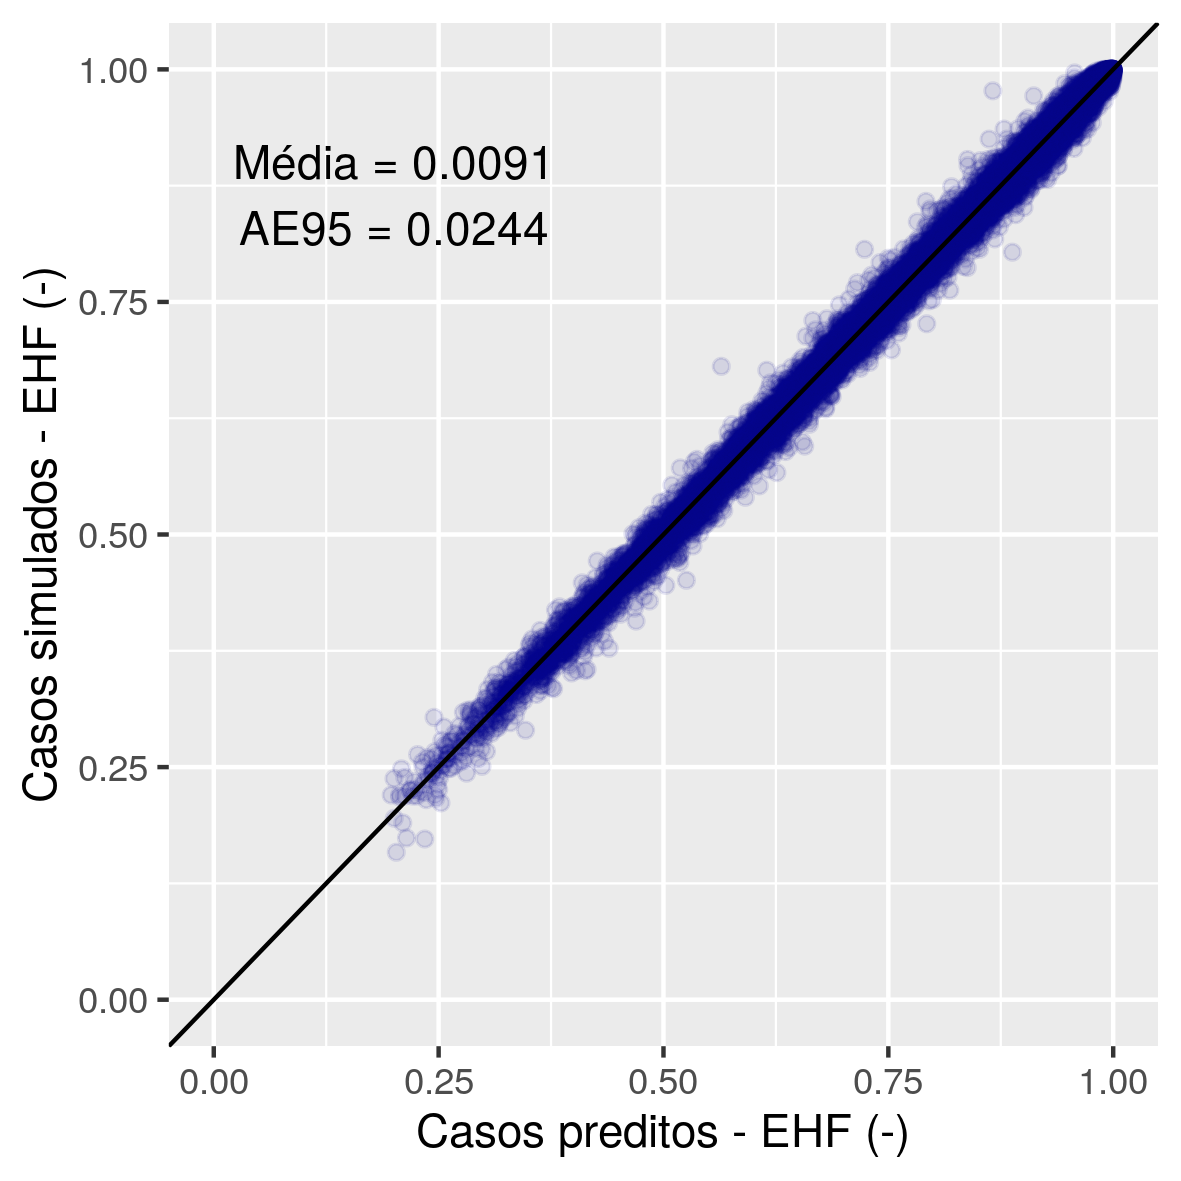
\includegraphics[width=1\linewidth]{img/ann_validation.png}
		\begin{center}
			\small{(a) Amostra de validação}
		\end{center}
	\end{minipage}%
	\begin{minipage}{.5\textwidth}
		\centering
		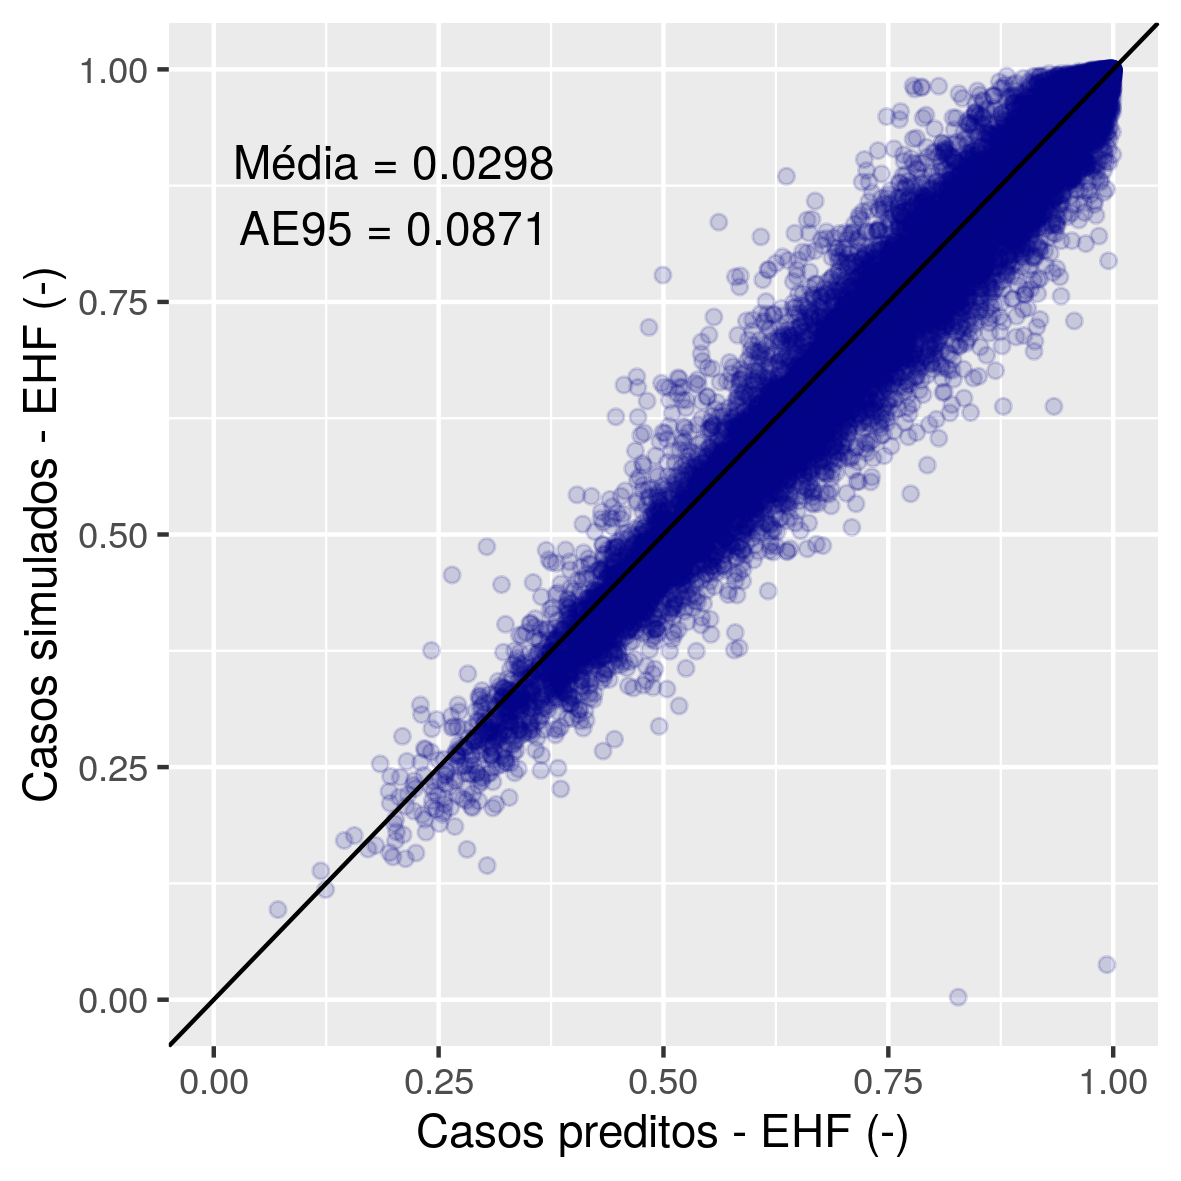
\includegraphics[width=1\linewidth]{img/ann_test.png}
		\begin{center}
			\small{(b) Amostra de teste}
		\end{center}
	\end{minipage}
	\label{fig:ann_validation}
\end{figure}

%\begin{figure}[H]
%	\centering
%	\caption{Condição de exposição das paredes e janelas}
%	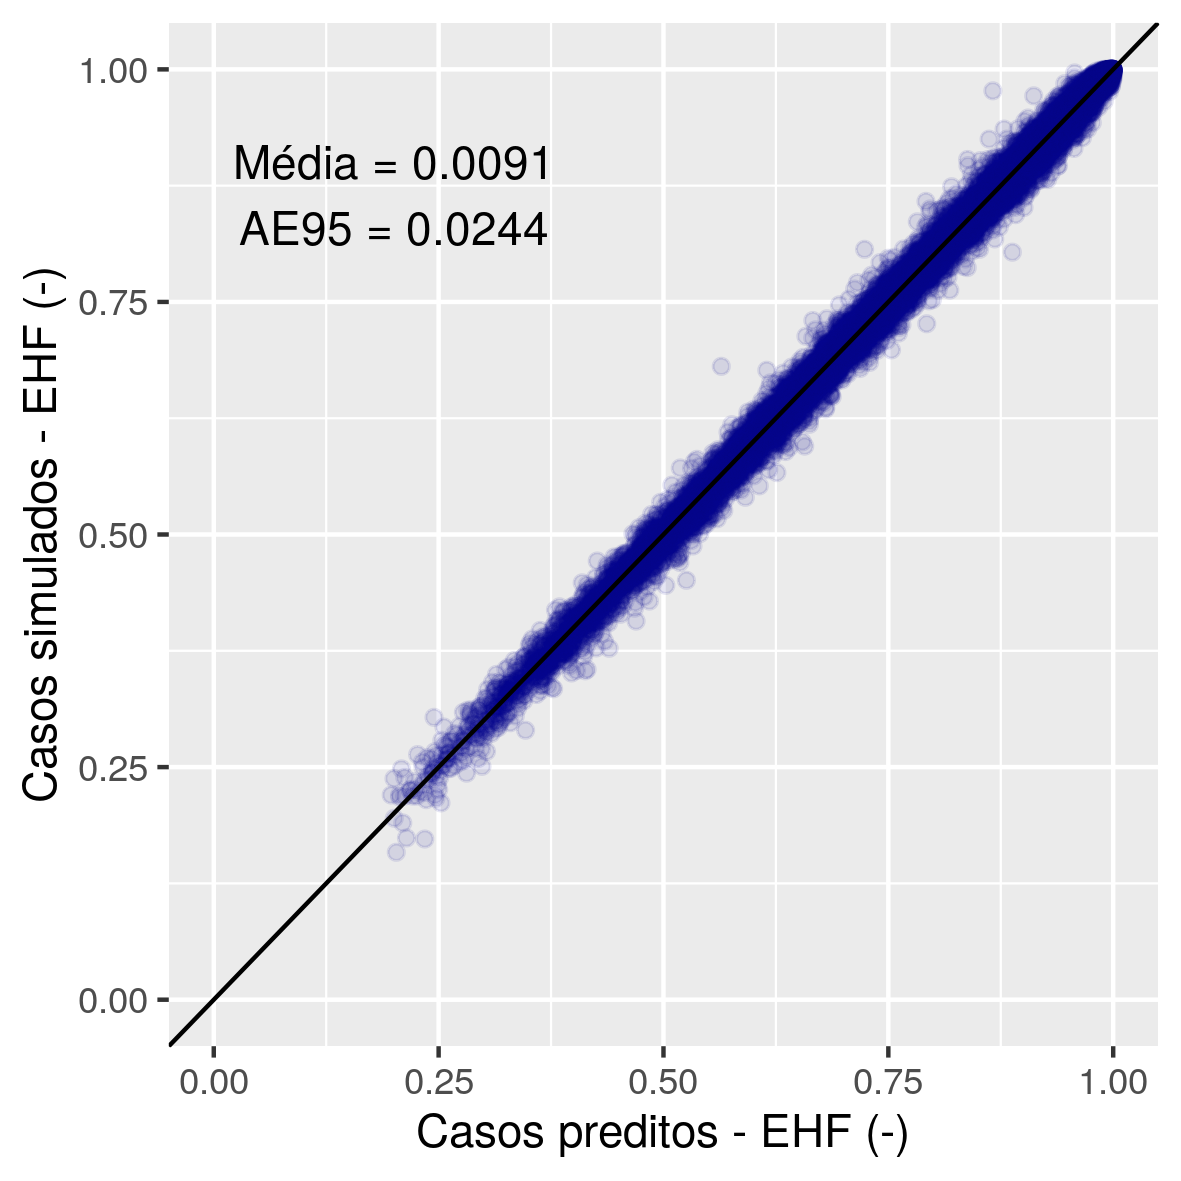
\includegraphics[width=.5\linewidth]{img/ann_validation.png}
%	\label{fig:ann_validation}
%\end{figure}

Para verificar as incertezas geradas nos resultados quando os parâmetros não incluídos como dados de entrada da \acrshort{ann} variam, outra amostra foi gerada para teste, com 20.000 casos.
A Figura \ref{fig:ann_validation}b apresenta o gráfico de pontos comparando os resultados de \acrshort{ehf} obtidos para as simulações e para as estimativas da \acrshort{ann}, a partir da base de dados gerada para verificar o impacto das incertezas no resultados. O erro absoluto médio do \acrshort{ehf} para os casos de validação foi 0,0298, com o \acrshort{ae95} igual a 0,0871.
No gráfico, é possível observar que os resultados para amostra de teste apresentam um enviesamento nas estimavas do \acrshort{ehf}, que retornam valores mais altos do que os obtidos pelas simulações. Essa diferença se faz mais expressiva em faixas de valores mais baixas de \acrshort{ehf}. Para os casos simulados com resultados de \acrshort{ehf} inferiores a 0,50, as estimativas de \acrshort{ehf} obtidas pela \acrshort{ann} são em média 0,0315 mais altas.

Os resultados obtidos pelo metamodelo desenvolvido apontam que a \acrshort{ann} é capaz de estimar adequadamente o conforto térmico em relação aos resultados simulados pelo programa EnergyPlus. 
Apesar das diferenças observadas entre os resultados preditos e simulados, os erros não são expressivos a ponto de impedir o uso da ferramenta.
Em situações em que há a necessidade de respostas rápidas, sem a possibilidade de utilizar-se programas de simulação computacional, como o EnergyPlus, a \acrshort{ann} desenvolvida pode ser aplicada, de maneira simples, para oferecer respostas relacionadas ao desempenho térmico de edifícios de escritório.

%\begin{figure}[H]
%	\centering
%	\caption{Condição de exposição das paredes e janelas}
%	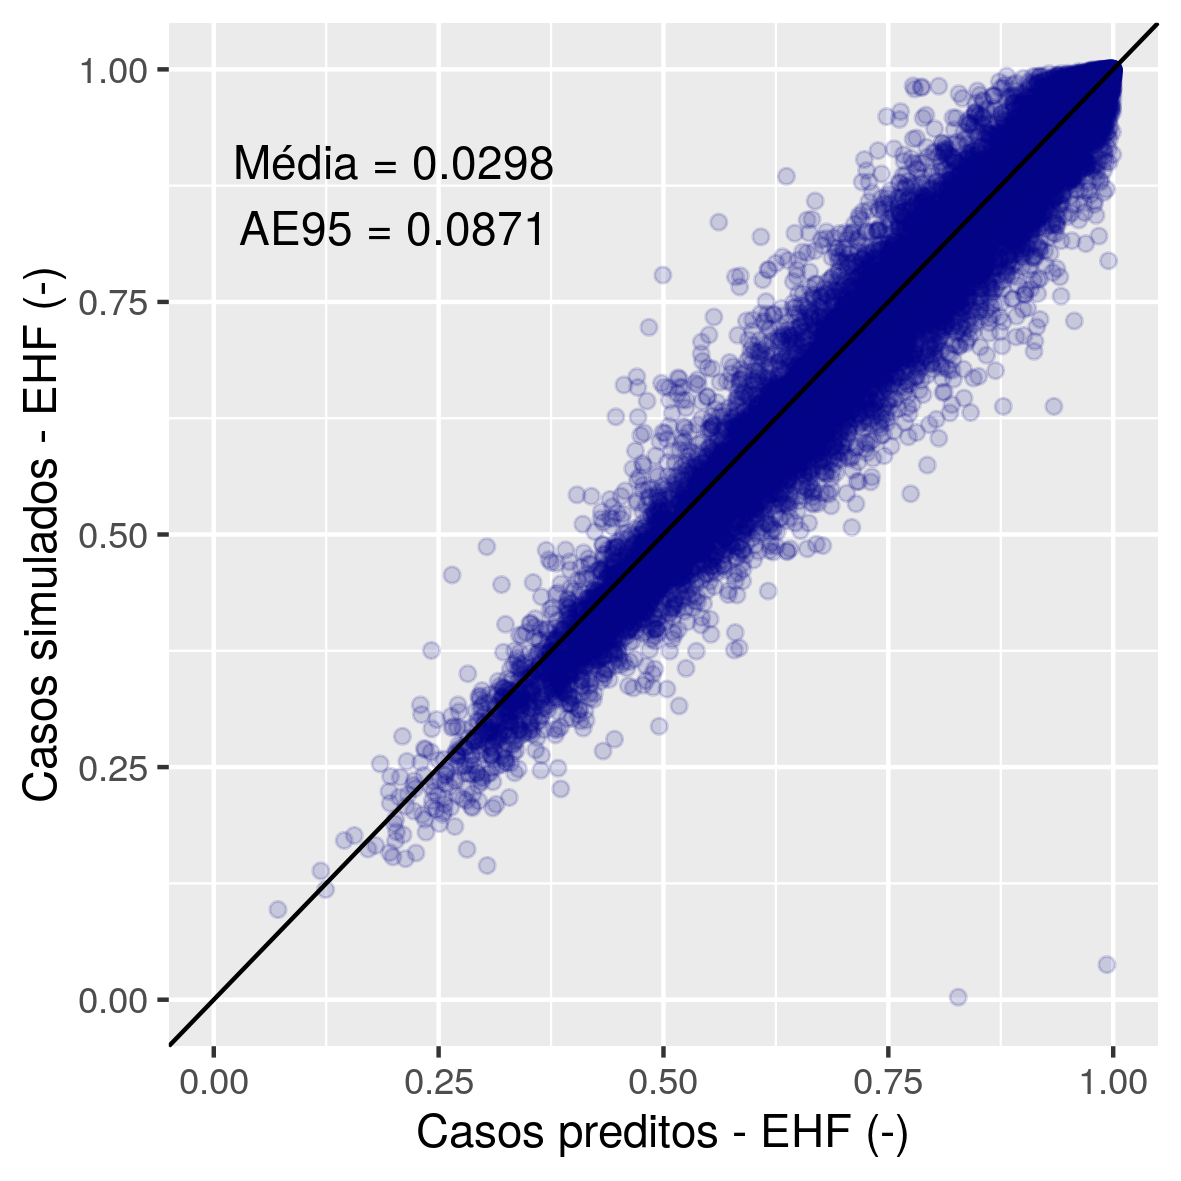
\includegraphics[width=.5\linewidth]{img/ann_test.png}
%	\label{fig:ann_sobol}
%\end{figure}